\documentclass[11pt, journal]{IEEEtran}

\usepackage{lipsum}
\usepackage[T1]{fontenc}
\usepackage{fouriernc}
\usepackage{cases}
\usepackage{amsmath}
\usepackage{amssymb}
\usepackage[noadjust]{cite}
\usepackage{hyperref}
\usepackage{multirow}
\usepackage{graphicx}
\usepackage{adjustbox}
\usepackage{makecell}
\usepackage[dvipsnames]{xcolor}
\usepackage{tikz}
\usepackage{lipsum}
\usepackage{listings}
\usepackage{fontawesome5}
\usepackage{tcolorbox}
\usepackage[dvipsnames]{xcolor}
\usepackage[ruled]{algorithm2e}
%\usepackage{caption}
%\usepackage{biblatex}

%\addbibresource{bibliography.bib}

\hypersetup{
    colorlinks=true,
    linkcolor=blue,
    anchorcolor=blue,
    urlcolor=blue,
    citecolor=blue
}

\definecolor{codeCOMMENT}{HTML}{649541}
\definecolor{codeSTRING}{HTML}{37864A}
\definecolor{codeKEY}{HTML}{C678DD}
\definecolor{codeFUNC}{HTML}{61AFEF}
\definecolor{codeVALUES}{HTML}{C69438}

\newcommand{\eq}{\; = \;}
\newcommand{\nwl}{

\vspace{11pt}

}
\newcommand{\centered}[2]{\begin{tabular}{#1} #2 \end{tabular}}

\lstdefinestyle{standstyle}{
    commentstyle=\color{codeCOMMENT},
    keywordstyle=\bfseries\color{codeKEY},
    numberstyle=\scriptsize\ttfamily\color{codeVALUES},
    stringstyle=\color{codeSTRING},
    basicstyle=\ttfamily\linespread{1}\scriptsize\color{black!80},
    breakatwhitespace=false,
    breaklines=true,
    captionpos=b,
    keepspaces=true,
    numbers=left,
    numbersep=5pt,
    showspaces=false,
    showstringspaces=false,
    showtabs=false,
    tabsize=4,
    xleftmargin=15pt,
}

\lstset{style=standstyle}

%\newfloat{Code}{htbp}{loa}

\DeclareMathAlphabet{\mathcal}{OMS}{zplm}{m}{n}
\DeclareMathOperator*{\argmax}{arg\,max}
\DeclareMathOperator*{\argmin}{arg\,min}

\newcommand{\norm}[1]{\left\lVert#1\right\rVert}
\newcommand\commentalg[1]{\textcolor{ForestGreen}{{\footnotesize #1}}}
\SetCommentSty{commentalg}

\title{$k$-means Is All You Need}
\author{Leonardo Biason ($2045751$) \quad Alessandro Romania ($2046144$) \quad Davide De Blasio ($2082600$)}

\begin{document}

\maketitle

\begin{abstract}
    The $k$-means algorithm is a well known clustering algorithm, which is often used in unsupervised learning settings. However, the algorithm requires to perform multiple times the same operation on the data, and it can greatly benefit from a parallel implementation, so that to maximize the throughput and reduce computation times. With this project, we propose some possible implementations, based on some libraries that are considered to be the \text{de-facto} standard when it comes to writing multithreaded or parallel code, and we will discuss also the results of such implementations
\end{abstract}

\begin{keywords}
    Sapienza, ACSAI, Multicore Programming
\end{keywords}
\nwl
%\begin{tcolorbox}[colback = Purple!20, colframe = Purple!40]
%    \begin{center}
%        \faIcon{github} Check our repository \href{https://www.github.com/ElBi21/PSEM-kmeans}{on GitHub}
%        \verb|ElBi21/PSEM-kmeans|
%    \end{center}
%\end{tcolorbox}

\section{Introduction}

When talking about clustering and unsupervised learning, it's quite common to hear about the $k$-means algorithm, and for good reasons: it allows to efficiently cluster a dataset of $d$ dimensions, and it employs the notion of convergence in order to do so. This, computationally speaking, means to repeat some operations over and over again until some stopping conditions are met.
\nwl
The algorithm is not perfect though, and presents some issues:
\begin{itemize}
    \item [1)] the algorithm is fast in clustering, but we cannot be certain that it clusters \textit{well};
    \item [2)] the algorithm doesn't work with non-linear clusters;
    \item [3)] the initialization can make a great impact in the final result.
\end{itemize}
\nwl
Many people prefer to use other clustering methods, such as the fitting of Gaussian Mixture Models. Albeit not being perfect, $k$-means still works well in simple, linear clusters. For the sake of this project, we are going to consider a vanilla $k$-means algorithm with Lloyd's initialization (the first $k$ centroids will be selected randomly).

\subsection{Algorithm structure}

The $k$-means algorithm can be described with the following pseudocode, where $X$ is the set of data points, $C = \{\mu_1, \; \mu_2, \; ..., \; \mu_k \}$ is the set of centroids and $Y$ is the set of assignments:

\begin{algorithm}
    \label{algkmeans}
    \LinesNumbered
    \tcp{Initialize the centroids}
    \For{$k$ in $[1, \; |C|]$}{
        $\mu_k \gets \text{a random location in the input space}$
    }
    \BlankLine
    \While{$\text{convergence hasn't been reached}$}{
        \tcp{Assign each point to a cluster}
        \For{$i$ in $[1, \; |X|]$}{
            $y_i \gets \argmin_k \left(\norm{\mu_k - x_i}\right)$ 
        }
        \BlankLine
        \tcp{Compute the new position of each centroid}
        \For{$k$ in $[1, \; |C|]$}{
            $\mu_k \gets \textsc{Mean}(\{ \; x_n : z_n = k \; \})$
        }
    }
    \tcp{Return the centroids}
    \Return $Y$

    \caption{$k$-means (Lloyd's initialization)}
\end{algorithm}

The algorithm consists of 4 main blocks:
\begin{itemize}
    \item the \textbf{initialization block}, where all the centroids will receive a starting, random position (as per Lloyd's method);
    \item the \textbf{assignment block}, where the Euclidean distance between a point and all centroids is computed, for all centroids. The point will be assigned to a cluster depending on the following operation:
    \[ \argmin_k \left(\norm{\mu_k - x_i}\right) \]

    \item the \textbf{update block}, where the position of the centroids is updated, and the new position of a centroid $\mu_k$ is equal to the mean of all the data points positions belonging to cluster $k$
\end{itemize}

\subsection{Sequential Code Bottlenecks}

For implementing the $k$-means algorithm, we will base all the codebase upon the project made from professors Diego García-Álvarez and Arturo Gonzalez-Escribano from the University of Valladolid. The code shown in this subsection is taken from their project, although slightly adapted for giving enough context in the code snippets.
\nwl
We described before the overall structure of the $k$-means algorithm: we will now proceed to examine its two main bottlenecks. As we can see from Algorithm \ref{algkmeans}, we have two main blocks that may cause performance issues: the \textbf{assignment block} and the \textbf{update block}.
\nwl
The first \textbf{for} block in the \textbf{initialization step} does not represent a major bottleneck, since it just needs to assign a random location to each of the $K$ centroids. It can be parallelized, but it won't help as much as parallelizing the two steps mentioned before.
\nwl
The second \textbf{for} block represents the \textbf{assignment step}, which is, unlike the initialization step, computationally expensive: for each point, the algorithm will have to compute the euclidean distance (here onwards denotes as $\ell_2$) between said point and all centroids $\mu_k \in C$, and select the lowest distance. This will determine the cluster of the point. In a C program, this may be accomplished with the following piece of code:
\nwl
\begin{lstlisting}[language = C]
int cluster;
// For each point...
for(i = 0; i < points_number; i++) {
    class = 1;
    minDist = FLT_MAX;
    // For each cluster...
    for(j = 0; j < K; j++) {
        // Compute the distance
        dist = l2_norm(&data[i*samples], &centroids[j*samples], samples);

        // If the distance is the lowest so far, replace it
        if(dist < minDist) {
            minDist = dist;
            class = j+1;
        }
    }
    
    // If the class is different from before, add a change to the counter
    if(classMap[i] != class) {
        changes++;
    }

    classMap[i]=class;
}\end{lstlisting}

Notice the presence of the two nested \textbf{for} loops: sequentially, they would take a time of $O(|X| \cdot |C|)$, which may be optimized just by taking a simple single instruction multiple data approach (indeed, with $m > 1$ different processes or threads, it would take a time of $O\left(\frac{|X| \cdot |C|}{m}\right)$ each, which is already better than the first option).
\nwl
The third \textbf{for} loop represents the update step, which also is computationally expensive: we would need to perform the mean of the coordinates of all the points belonging to a cluster $\mu_k$. This implies that all the coordinates of the points must be first summed, and then averaged on the number of points being classified to $\mu_k$. An implementation in the C language would look like the following:
\nwl
\begin{lstlisting}[language = C]
// For each point...
for (i = 0; i < lines; i++) {
    point_class = classMap[i];
    // Add 1 to the points classified for class k
    pointsPerClass[point_class - 1] += 1;

    // For each dimension...
    for(j = 0; j < samples; j++) {
        // ...add it to a table for summing and averaging
        auxCentroids[(point_class - 1) * samples + j] += data[i * samples + j];
    }
}

for (i = 0; i < K; i++) {
    for (j = 0; j < samples; j++) {
        // Average all dimensions
        auxCentroids[i * samples + j] /= pointsPerClass[i];
    }
}

maxDist = FLT_MIN;
for (i = 0; i < K; i++) {
    // Compute the moving distance, as a convergence check
    distCentroids[i] = euclideanDistance(&centroids[i * samples], &auxCentroids[i * samples], samples);
    if (distCentroids[i] > maxDist) {
        maxDist = distCentroids[i];
    }
}\end{lstlisting}

\section{Parallelizing with MPI}

The Message Passing Interface (MPI) is a standardized, portable framework that enables parallel computation across distributed memory systems. These systems, typically clusters of interconnected computers, do not share a common memory. Each process operates on its local memory and must explicitly communicate with others by sending and receiving messages. MPI achieves parallelism through process-based communication, distributing both data and tasks among multiple processes.
\nwl
Achieving efficient parallel performance in MPI programs requires attention to two critical factors:

\begin{itemize}
    \item [1)] Balancing the workload across processes;
    \item [2)] Minimizing the frequency of message passing.
\end{itemize}
\nwl
Both factors are crucial for scalable and high-performance parallel applications. We here show how these optimizations are implemented in this $k$-means clustering algorithm. By deafult, the $k$-means clustering program follows a Globally Parallel, Locally Sequential (GPLS) model. This means that the critical initialization and termination tasks are handled by rank 0, while the looping part of the algorithm is entirely parallelized. 

\subsection{Design of the program}

\noindent \textbf{Initialization Phase}

The initialization phase is where workload balancing decisions are made. Rank 0 reads the input data from a file (as only rank 0 has access to the file). The input data (points) is broadcast to all processes using \texttt{MPI\_Scatterv}. The points remain fixed throughout the execution, enabling a single communication step to distribute data efficiently. The Centroids are randomly generated by rank 0. These centroids are then broadcasted to all processes.
\nwl
\noindent \textbf{Point assignment}

Each process works on its local points with its local \texttt{classMap}. This assignment step is fully parallel, as each process handles its portion of the points independently. Assignment changes are accumulated locally and reduced globally, by using the \texttt{MPI\_Iallreduce} collective for checking, at the end of each iteration, the termination conditions.
\nwl
\noindent \textbf{Centroids update}

Once points are assigned, each process computes its local partial sums for each centroid and the number of points in each cluster. These partial results are aggregated across all processes using \texttt{MPI\_Allreduce}, ensuring globally consistent centroid values with fast communication. Each process then updates its locally assigned centroids based on the reduced global values, distributing the workload evenly among processes. The maximum distance between old and updated centroids is calculated locally and reduced globally using \texttt{MPI\_Allreduce} to check for termination conditions. After these checks, an \texttt{MPI\_Allgatherv} operation gathers all local
centroids, preparing them for the next iteration.
\nwl
\noindent \textbf{Termination phase}

In the termination phase, local point assignments (the output of the $k$-means algorithm) are gathered by the rank 0 process using \texttt{MPI\_Gather}. Finally, all processes free their allocated memory, and the algorithm terminates.

\section{Parallelizing with OpenMP}

As a mean of enhancing the performance of the $k$-means algorithm, we made use of the multi-thread library OpenMP. OpenMP is a widely-used API for multi-platform shared-memory parallel programming. Our primary goal was to leverage multiple CPU cores to expedite the computationally intensive parts of the algorithm: the \textbf{cluster assignment} and \textbf{centroid update} steps. The number of threads can be optionally specified as a parameter; if not provided, a default value (i.e. 8 threads) is used for parallel execution.
We now show how we approached the parallelization of the program, and the advantages of taking certain design decisions.
 
\subsection{OpenMP Implementation Approach}

\noindent \textbf{Cluster assignment}

The cluster assignment step is inherently parallelizable since each data point can be processed independently. We made use of the \texttt{\#pragma omp parallel for} directive to distribute the loop iterations across multiple threads. Said directive has been accompanied by the following clauses:

\begin{itemize}
    \item \texttt{reduction(+ : changes)}: the \textbf{reduction clause} safely aggregates the total number of cluster reassignments across threads. This avoids race conditions by creating thread-private copies of \texttt{changes} that are combined after the loop;
    \item \texttt{schedule(dynamic, 16)}: the \textbf{dynamic scheduling} clause improves load balancing by allowing threads to dynamically claim "chunks" of 16 iterations.
\end{itemize}
\nwl
\noindent \textbf{Centroid update}

The centroid update step involves two parallel phases: gathering cluster sums and averaging the centroids coordinates. However, the program could incur in race conditions. In order to address them, we made use of OpenMP's concepts of privatization and synchronization:
\begin{itemize}
    \item \textbf{Privatization with local buffers}: Each thread maintains private copies of two buffers, namely \texttt{local\_pointsPerClass} (count of points assigned to the cluster) and \texttt{local\_auxCentroids} (cumulative sum of data points for each cluster). This eliminates races during local accumulation, as threads operate on isolated data;
    \item \textbf{Critical Section for global aggregation}: After local accumulation, a \texttt{\#pragma omp critical} region safely merges thread-local results into global \texttt{pointsPerClass} and \texttt{auxCentroids}. While critical sections incur synchronization overhead, they are used sparingly here once per thread in order to minimize contention;
    \item \textbf{Parallel mean calculation}: The final centroid normalization loop (\texttt{\#pragma omp parallel for}) parallelizes the division by \texttt{pointsPerClass}, avoiding race conditions since each cluster is processed independently.
\end{itemize}
\nwl
An alternative approach that we experimented with uses the reduction feature to eliminate the need for explicit synchronization.
\nwl
\begin{lstlisting}[language = C]
#pragma omp parallel for reduction(+ : pointsPerClass[ : K], auxCentroids[ : K * samples])
		for (i = 0; i < lines; i++)
		{
			int class = classMap[i] - 1;
			pointsPerClass[class]++;
			for (int j = 0; j < samples; j++)
			{
				auxCentroids[class * samples + j] += data[i * samples + j];
			}
		}\end{lstlisting}
\nwl
The reduction clause automates the process of merging thread-local results into shared variables. By reducing both \texttt{pointsPerClass} and \texttt{auxCentroids}, the need for a critical section is removed, potentially lowering synchronization overhead.
However, we chose the original approach with explicit privatization and critical regions to demonstrate proficiency with OpenMP synchronization and race condition management. 
\nwl
The maximum centroid displacement (\texttt{maxDist}) is computed serially. While this loop could be parallelized using the \texttt{\#pragma omp parallel for reduction(max : maxDist)} directive, we retained the serial approach for simplicity, as its computational cost is negligible compared to other steps and because the number of clusters $k$ is typically small, the overhead associated with parallelization outweighs the potential performance gains.

\subsection{Solutions Implemented}

\begin{itemize}
    \item \textbf{Reduction for Scalars}: The \texttt{changes} variable uses a \texttt{reduction} clause, which is more efficient than atomic operations for scalar summation. OpenMP handles private copies and post-loop merging automatically.
    \item \textbf{Privatization and Critical Sections}: For array/matrix updates (i.e., \texttt{auxCentroids}), thread-local buffers reduce the need for fine-grained synchronization. The critical section ensures safe aggregation with minimal overhead, as it is invoked only once per thread.
    \item \textbf{Atomic Operations vs. Critical Regions}: While atomic operations (i.e., \texttt{\#pragma omp atomic}) could replace the critical section for scalar increments (\texttt{pointsPerClass}), they would be inefficient for matrix additions (\texttt{auxCentroids}) due to repeated fine-grained locking. Privatization strikes a better balance between correctness and performance.
\end{itemize}

\subsection{Performance Considerations}

\begin{itemize}
    \item \textbf{Critical Section Overhead}: The single critical section per thread during centroid aggregation has negligible cost compared to the computational work, as merging local buffers is a minor operation.
    \item \textbf{Memory Efficiency}: Privatizing per thread the \texttt{local\_auxCentroids} buffer increases memory usage proportionally to the number of threads. However, this is manageable for moderate thread counts and cluster sizes.
    \item \textbf{Dynamic Scheduling Trade-off}: While dynamic scheduling improves load balancing, it introduces overhead for chunk management. A chunk size of 16 was empirically chosen to balance parallelism and scheduling latency.
\end{itemize}

\section{Parallelizing with CUDA}

In recent years, we have seen how GPUs play crucial roles when it comes to parallelizing a program with multiple threads. Indeed, the model proposed by NVIDIA for its CUDA platforms (namely, the Single-Thread Multiple-Data model) turned out to be very efficient, by allowing notable speed-ups and augmentation of the throughput. Here follows an explanation of how we decided to design a possible CUDA implementation.

\subsection{Designing the parallel structure}

As we have shown in Algorithm \ref{algkmeans}, the $k$-means algorithm can be logically split into two steps: the assignment step and the update step. However, while logically this division may sound reasonable, it is not appropriate for the STMD model that NVIDIA has at the core of its devices. This is because of the needed data for the two steps: the assignment step needs to work only with the data points, but can be parallelized by splitting the data into multiple parts; the update step instead needs to work with both all the data and all the centroids, so parallelizing the step as a whole becomes quite hard.
\nwl
A simpler approach would be to split the update step in two parts, one that uses a fraction of the points, and the other that uses a fraction of the centroids. This would create in total three parallelization steps. However, the assignment step and the first part of the update step can be merged together, since they both need to work with part of the data. This is the reason why we decided to implement the program with two kernels, called respectively \verb|step_1_kernel| and \verb|step_2_kernel|, where the first kernel can be considered as points-based and the second kernel as centroids-based.

\subsection{Program parameters and custom atomicMax}

We decided to organize the threads in two dimensional blocks of $32 \times 32$ threads, and the blocks are instead organized in a one dimensional grid. The size of the grid depends on the called kernel: usually, we have that $|X| \gg |C|$, so it's pointless for CUDA to reserve a grid of threads for the centroids that has the same size of the grid of the points. Indeed, the grids' single dimensions are dynamic, and are computed as follows:

\[ \texttt{points\_grid\_size} \; = \; \frac{\left| X \right|}{32 \times 32} + 1 \]
\[ \texttt{centroids\_grid\_size} \; = \; \frac{k}{32 \times 32} + 1 \]

The program makes also use of a custom function, called \verb|custom_atomic_max()|. This function has been implemented because it allows us to perform an \verb|atomicMax()|-like function for \verb|float| numbers, which would not be normally possible with the built-it CUDA function. We here show the function as a whole:
\nwl
\begin{lstlisting}[language = C]
__device__ float custom_atomic_max(float* value_address, float val) {
    int* address_as_int = (int*) value_address;
    int old = *address_as_int, assumed;
    do {
        assumed = old;
        old = atomicCAS(address_as_int, assumed, __float_as_int(fmaxf(val, __int_as_float(assumed))));
    } while (assumed != old);
    return __int_as_float(old);
}\end{lstlisting}
\nwl
The idea of the function is that CUDA tries continuously to perform an \verb|atomicCAS()| operation, which in turns performs atomically the following check:
\begin{center}
    \scriptsize
    \verb|old_value == to_compare ? new_value : old_value|
\end{center}

The function will exit only when the value in the specified address is equal to the one that the program expects to be there, before performing the atomic transaction. This is important, so that to avoid that the function overwrites any unintentional value.

\subsection{Analysis of the kernels}

As we mentioned previously, we are making use of two kernels: \verb|step_1_kernel| and \verb|step_2_kernel|. In both kernels, all operations that act on the global memory are performed atomically, which avoid potential race conditions. We here show how both kernels work, alongsize their code snippets.
\nwl
The first kernel is called on all the data, and each point is assigned to a thread. First, a preliminary check is performed, to make sure that each thread is assigned to a valid point. While the \verb|if| statement may seem like a possible cause of warp divergence, it doesn't actually impact that much. Indeed, we would only discard part of the final block of kernels, while all the previous blocks are fully used.
\nwl
Then, each thread will compute the $\ell_2$ norm of each point for all centroids, and will store the class to which each point will be assigned into the \verb|class_int| variable. If a change from the previous class assignment is detected, the number of changes will increase. After that, each thread will proceed to sum the coordinates of its assigned point into the auxiliary centroids matrix. The coordinates will then be averaged in the second kernel.
\nwl
\begin{lstlisting}[language = C]
__global__ void step_1_kernel(float* data, float* centroids, int* points_per_class, float* aux_centroids, int* class_map, int* changes_return) {

// Compute global thread index
int thread_index = (blockIdx.y * gridDim.x * blockDim.x * blockDim.y) + (blockIdx.x * blockDim.x * blockDim.y) + (threadIdx.y * blockDim.x) + threadIdx.x;

if (thread_index < gpu_n) {
    int class_int = class_map[thread_index];
    float min_dist = FLT_MAX;
    
    // For each centroid...
    for (int centroid = 0; centroid < gpu_K; centroid++) {
        float distance = 0.0f;

        // Compute the euclidean distance
        euclideanDistance(&data[thread_index * gpu_d], &centroids[centroid * gpu_d], gpu_d, &distance);

        // If distance is smaller, replace the distance and assign new class
        if (distance < min_dist) {
            min_dist = distance;
            class_int = centroid + 1;
        }
    }

    // If the class is different, add one change and write new class
    if (class_map[thread_index] != class_int) {
        atomicAdd(changes_return, 1);
    }
    
    // Map the value to the class map
    class_map[thread_index] = class_int;

    int class_assignment = class_map[thread_index];
    int point_index = class_assignment - 1;

    atomicAdd(&(points_per_class[point_index]), 1);

    for (int dim = 0; dim < gpu_d; dim++) {
        int index = point_index * gpu_d + dim;
        atomicAdd(&aux_centroids[index], data[thread_index * gpu_d + dim]);
    }
}}\end{lstlisting}

The second kernel performs the same check as \verb|step_1_kernel| on each thread, to ensure that all threads are mapped to a valid centroid. After that, all threads will compute, for each dimension of the centroids, the average coordinate. Once computed, each thread will then perform the $\ell_2$ norm between the previous centroid and the new one, so that to compute the \verb|max_distance| variable, needed for convergence. Finally, via the use of the \verb|custom_atomic_max()| function, the gratest distance is stored in memory.
\nwl
\begin{lstlisting}[language = C]
__global__ void step_2_kernel(float* centroids_table, float* centroids, int* points_per_class, float* max_distance) {
// Index of the thread
int thread_index = (blockIdx.y * gridDim.x * blockDim.x * blockDim.y) + (blockIdx.x * blockDim.x * blockDim.y) +
                        (threadIdx.y * blockDim.x) +
                        threadIdx.x;

if (thread_index < gpu_K) {
    float distance;
    // For each dimension...
    for (int d = 0; d < gpu_d; d++) {
        centroids_table[thread_index * gpu_d + d] /= (float) points_per_class[thread_index];
        // Compute Euclidean distance (l_2 norm) to check for maximum distance
        distance += pow((centroids[thread_index * gpu_d + d] - centroids_table[thread_index * gpu_d + d]), 2);
    }

    // Perform sqrt of distance
    //distance = sqrt(distance);

    // Exchange atomically, disregard old value
    custom_atomic_max(max_distance, distance);
}}
\end{lstlisting}

After executing the second kernel, the program continues repeating in loop the two kernels until one of the convergence conditions is met.

\section{Interlacing Multi-processing with Multi-threading}

So far, we implemented various solutions for our programs, which employed either multi-processing or multi-threading parallelism techniques, without using both approaches at the same time. However, these techniques are not mutually exclusive, and can be mixed together in order to achieve better performances. In fact, in high performance computing tasks, multi-process techniques are used within clusters to connect nodes and coordinate them, while multi-threading are used for performing computations, given the directives of the master process(es).
\nwl
In this section we will show how the two multi-threading approaches that we previously considered (namely, OpenMP and CUDA) can be combined with the famous multi-processing library MPI. Furthermore, we will show another implementation with the PThreads library.

\subsection{MPI and OpenMP}

The hybrid MPI $+$ OpenMP implementation of the $k$-means clustering algorithm leverages both distributed and shared memory parallelism to enhance performance and scalability. Our parallelization strategy can be described with three main key points:
\nwl
\noindent \textit{Two-level parallelism}
\begin{itemize}
    \item MPI distributes data across processes (coarse-grained parallelism) with \texttt{MPI\_Scatterv}, a vector scattering collective, while OpenMP parallelizes loops within each process (allowing for a much fine-grained parallelism);
    \item Thread safety: all the processes are initialized with \texttt{MPI\_THREAD\_FUNNELED}, so that to restrict MPI calls to the main thread.
\end{itemize}
\nwl
\noindent \textit{Asynchronous communication}

The non-blocking reduce operation \texttt{MPI\_Ireduce} aggregates cluster reassignment counts while centroid updates proceed, allowing to overlap communication and computation.
\nwl
\noindent \textit{Hybrid reductions}
\begin{itemize}
    \item OpenMP sets thread-local buffers in order to avoid intra-node races. More specifically, the \texttt{local\_pointsPerClass} and the \texttt{local\_auxCentroids} buffers;
    \item Global aggregations via \texttt{MPI\_Allreduce} ensures consistent centroid states across nodes.
\end{itemize}
\nwl
\begin{lstlisting}[language=C]
#pragma omp parallel  // Thread-local accumulation
{ 
    int *local_pointsPerClass = calloc(K, sizeof(int)); 
    float *local_auxCentroids = (float *)calloc(K * samples, sizeof(float));
    // ...
}

// Global sync
MPI_Allreduce(MPI_IN_PLACE, pointsPerClass, K, MPI_INT, MPI_SUM, MPI_COMM_WORLD); 
MPI_Allreduce(MPI_IN_PLACE, auxCentroids, K * samples, MPI_FLOAT, MPI_SUM, MPI_COMM_WORLD);\end{lstlisting}
\nwl
A major concern while designing this application was also ensuring that an efficient \textbf{data distribution} system was in place. We show, in the following two key points, how we tackled this problem:
\nwl
\noindent \textit{Balanced workloads}
\begin{itemize}
    \item The \texttt{MPI\_Scatterv} collective allows to split data into chunks, adjusted via two parameters: \texttt{sendcounts} and \texttt{displs}. Said collective is capable of handling uneven divisions, ensuring balanced workloads even when the total data points (\texttt{lines}) are not evenly divisible by the number of processes.
    \item Each process computes locally the updates for a subset of centroids. These partial updates are then gathered from all processes and redistributed to ensure that every process has the complete and updated set of centroids for the next iteration, using \texttt{MPI\_Allgatherv}. We report here the full collective call:
\begin{lstlisting}[language = C]
MPI_Allgatherv(local_centroids, local_k * samples, MPI_FLOAT, centroids, centroid_sendcounts, centroid_displs, MPI_FLOAT, MPI_COMM_WORLD);
\end{lstlisting}
\end{itemize}
\nwl
\noindent \textit{Final result aggregation}

After convergence, the \texttt{MPI\_Gatherv} collective reconstructs the global cluster assignments on the root process. Each process sends its own \texttt{local\_classMap} (containing classifications for its local data subset), and the root process assembles them into \texttt{classMap} using the precomputed \texttt{recvcounts} and \texttt{rdispls} offsets. Below the code snippet, which shows how the \texttt{MPI\_Gatherv} call was assembled, we give more precise definitions regarding the two offsets aforementioned:
\nwl
\begin{lstlisting}[language = C]
// Gather local classifications into root's classMap
MPI_Gatherv(local_classMap, local_lines, MPI_INT, classMap, recvcounts, rdispls, MPI_INT, 0, MPI_COMM_WORLD);
\end{lstlisting}
\nwl
\begin{itemize}
    \item \texttt{recvcounts}: array specifying the number of elements received from each process (matches \texttt{sendcounts} from initial scatter);
    \item \texttt{rdispls}: offsets in \texttt{classMap} where each process' data is stored.
\end{itemize}
\nwl
These offsets ensures efficient reconstruction of the global result without requiring intermediate storage on worker processes.
\nwl
\noindent \textbf{Memory efficiency}
\begin{itemize}
    \item Each process stores only its local data (\texttt{local\_points}) and centroid subset (\texttt{local\_centroids}).
    \item Thread-local buffers minimize shared memory contention without atomic operations.
\end{itemize}
\end{itemize}
\nwl
How did we approach \textbf{synchronization and termination}? %TODO
\nwl
\noindent \textbf{Convergence check}
\begin{itemize}
    \item OpenMP's \texttt{reduction(max:local\_maxDist)} computes per-process centroid displacements.
    \item \texttt{MPI\_Reduce} finds the global maximum displacement for termination decisions.
\end{itemize}
\nwl
\noindent \textbf{Termination broadcast}

Root process evaluates conditions and broadcasts \texttt{terminate} flag via \texttt{MPI\_Bcast}, ensuring synchronized loop exits.

\subsection{MPI + PThreads}

In order to further exploit both inter-node and intra-node parallelism, we developed a hybrid MPI $+$ PThreads implementation of the $k$-means clustering algorithm. In this design, MPI is used for data distribution, inter-process communication, and global reductions, while PThreads are employed within each MPI process to perform fine-grained parallel computations on multi-core architectures. This section describes our design choices, synchronization strategies, and performance considerations for the MPI $+$ PThreads approach.
\nwl
\noindent \textbf{Hybrid Implementation Overview}

The overall structure of the algorithm remains similar to the pure MPI implementation. We here list the main steps.

\subsubsection{Data Distribution} the root process reads the input file and determines the total number of data points and their dimensions. MPI collective operations (e.g., \texttt{MPI\_Scatterv}) are used to distribute chunks of the data among processes. Each process stores only its local subset of data, which helps in reducing per-node memory usage.
\nwl
\subsubsection{Local Computation with PThreads} within each MPI process, two computationally intensive steps are parallelized with PThreads:
\begin{itemize}
    \item \textbf{Cluster Assignment}: each process spawns a number of threads (configurable via a command-line parameter, with a default of 8 threads) to independently assign local data points to the nearest centroid. Each thread is responsible for a contiguous block of data points. The thread function (\texttt{assign\_points\_thread}) computes the squared Euclidean distance from each point to all centroids and updates the cluster assignment if a closer centroid is found.
    \item \textbf{Centroid Accumulation}: after assignment, a second round of PThreads is created to accumulate partial sums of point coordinates and counts for each cluster. The thread function (\texttt{centroid\_accumulate\_thread}) uses thread-private arrays (\texttt{partial\_counts} and \texttt{partial\_centroids}) to prevent race conditions during local accumulation. These partial results are later merged into global local accumulators.
\end{itemize}
\nwl
\subsubsection{Global Reductions and Centroid Update} Once the local contributions are computed, MPI collective operations (e.g., \texttt{MPI\_Allreduce} and \texttt{MPI\_Allgatherv}) are used to sum the centroid contributions and update the centroids across all processes. A non-blocking reduction (\texttt{MPI\_Iallreduce}) is employed to aggregate the number of changes in point assignments, overlapping communication with the centroid update computations.
\nwl
\subsubsection{Termination and Result Collection} the algorithm iterates until one of the stopping criteria is met. Finally, \texttt{MPI\_Gatherv} is used to collect the final cluster assignments from all processes.
\nwl
\noindent \textbf{PThreads Design Choices}

The design of the PThreads layer was carefully crafted to ensure efficient intra-node parallelism while minimizing synchronization overhead:

\begin{itemize}
    \item \textbf{Data Partitioning}: each MPI process divides its local data points evenly among the available threads. If the number of points is not evenly divisible by the number of threads, the extra points are distributed among the first few threads. This dynamic partitioning ensures a balanced workload.
    
    \item \textbf{Thread-Private Buffers}: during the centroid accumulation phase, each thread uses its own buffers (\texttt{partial\_counts} and \texttt{partial\_centroids}) to sum the contributions from its assigned data points. This strategy avoids fine-grained synchronization (e.g., using atomics or locking on each array update) and limits the need for critical sections to a single merge phase performed after all threads complete.
    
    \item \textbf{Assignment Function}: the \texttt{assign\_points\_thread} function processes a block of points independently. For each point, the thread computes the squared Euclidean distance to every centroid and updates the point's class if a closer centroid is found. The local change counter is updated in a thread-private variable to be merged later, reducing contention.
    
    \item \textbf{Centroid Merge}: once all threads finish the accumulation phase, the main thread aggregates the thread-local partial sums. The merged arrays are then used in a global MPI reduction to update the centroids.
\end{itemize}
\nwl
The following code snippet shows how PThreads has been employed for both point and centroids assignment:

\begin{lstlisting}[language = C]
pthread_t assign_threads[threads];
assign_thread_data_t assign_data[threads];
int points_per_thread = local_n / threads;
int extra = local_n % threads;
int current_start = 0;

for (int t = 0; t < threads; t++) {
    // [...] Store into assign_data, for each thread, the needed data
}

int local_changes = 0;
for (int t = 0; t < threads; t++) {
    pthread_join(assign_threads[t], NULL);
    local_changes += assign_data[t].local_changes;
}
\end{lstlisting}

\noindent \textbf{MPI Integration and Synchronization}

The MPI layer orchestrates the global coordination among processes, complementing the intra-process parallelism provided by PThreads. Key aspects of the MPI integration include:

\begin{itemize}
    \item \textbf{Balanced Data Distribution}: Data points are distributed to processes using \texttt{MPI\_Scatterv}. Each process computes its local number of points, and residual points (if any) are distributed evenly to avoid load imbalance.
    
    \item \textbf{Global Reductions}: The number of changes in cluster assignments is aggregated across processes using a non-blocking reduction (\texttt{MPI\_Iallreduce}). Similarly, partial centroid contributions computed by PThreads are merged across processes with \texttt{MPI\_Allreduce} to obtain the global sums and counts needed for centroid updates.
    
    \item \textbf{Centroid Synchronization}: After local updates, \texttt{MPI\_Allgatherv} is used to collect the updated centroids from all processes. This collective ensures that every process starts the next iteration with the same, globally consistent centroid values.
    
    \item \textbf{Final Aggregation}: Once convergence is reached, \texttt{MPI\_Gatherv} collects the final cluster assignments from all MPI processes, reconstructing the complete clustering result.
\end{itemize}

This hybrid approach effectively overlaps communication with computation, as the MPI non-blocking routines allow PThreads to continue working while global reductions are in progress. By combining MPI for coarse-grained distribution and PThreads for fine-grained parallelism, the implementation achieves scalable performance on multi-node, multi-core systems.

\subsection{MPI and CUDA}

???

\section{Performance Analysis}

We will now proceed to show the results of each implementation, by considering both the speed-up of the program and the relative efficiency. For all implementations, we used a number of processes $p$ and threads $t$ such that $p, \; t \in [2, 12]$. 

\subsection{MPI}

\begin{figure}
    \label{stats_mpi}
    \centering
    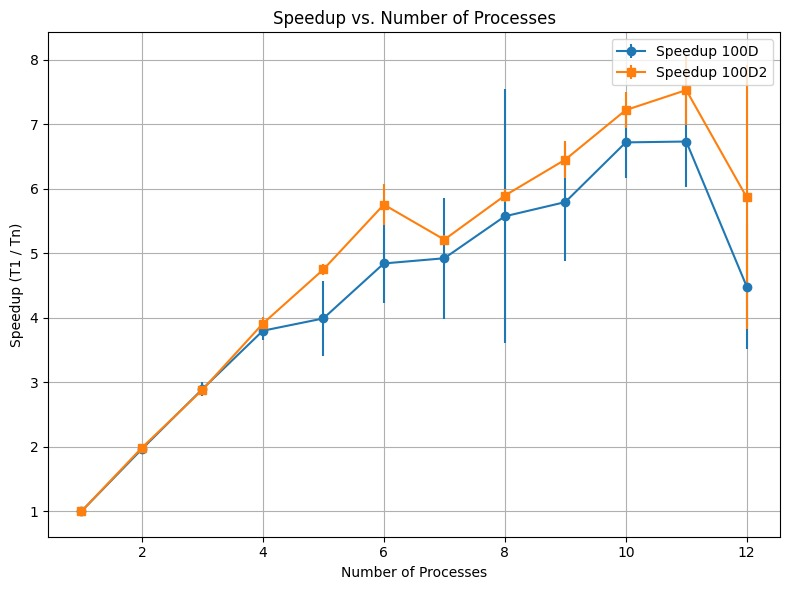
\includegraphics[width = 0.49\linewidth]{imgs/mpi_speedup.jpeg}
    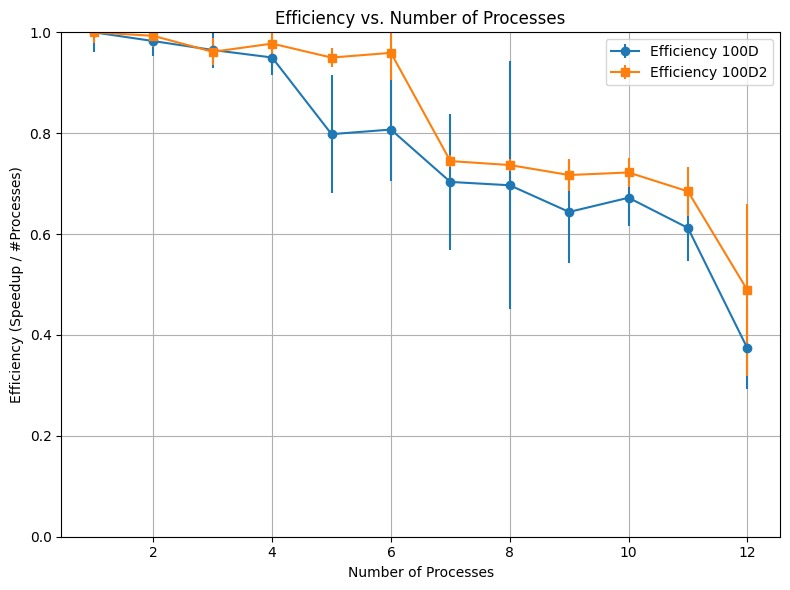
\includegraphics[width = 0.49\linewidth]{imgs/mpi_eff.jpeg}
    \\
    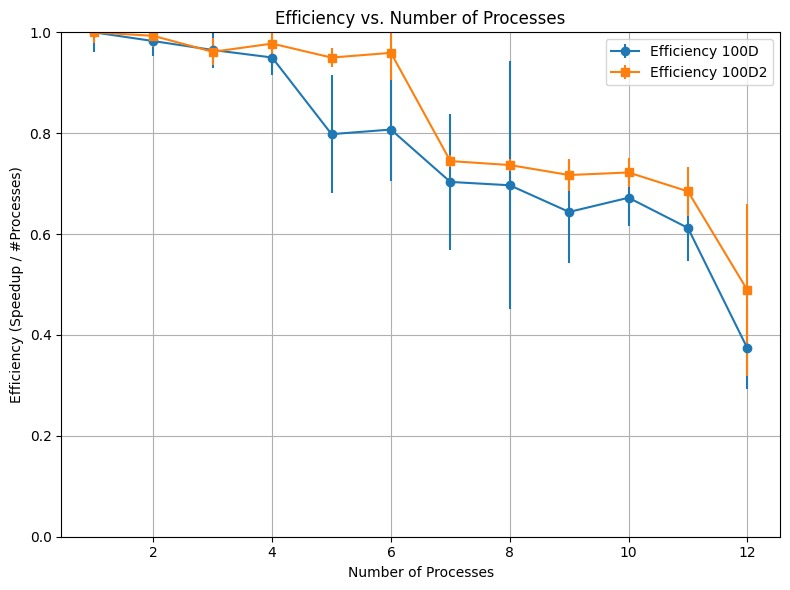
\includegraphics[width = 0.49\linewidth]{imgs/mpi_eff.jpeg}
    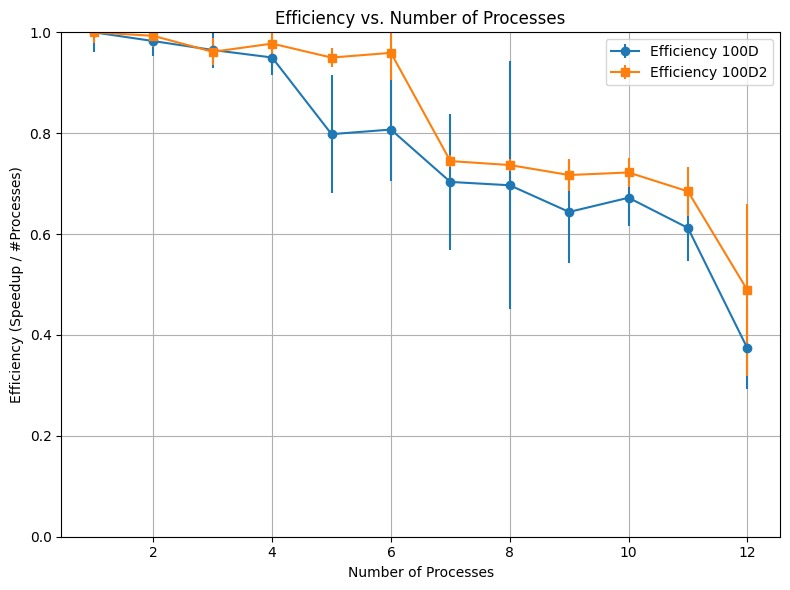
\includegraphics[width = 0.49\linewidth]{imgs/mpi_eff.jpeg}
    \\
    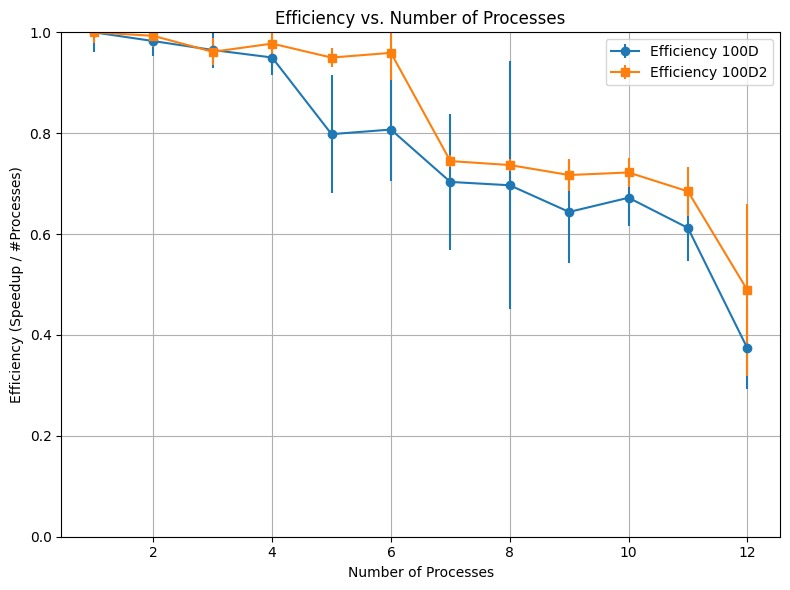
\includegraphics[width = 0.49\linewidth]{imgs/mpi_eff.jpeg}
    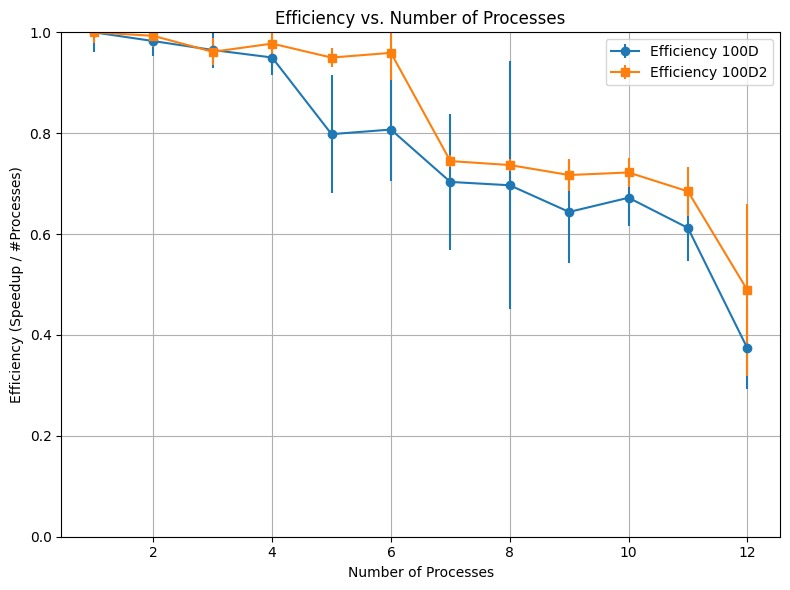
\includegraphics[width = 0.49\linewidth]{imgs/mpi_eff.jpeg}
    \caption{On the left, the speedups of MPI (above), OpenMP (middle) and CUDA (bottom), with different numbers of processes / threads; on the right, the relative efficiency}
\end{figure}

With MPI, we noticed that by augmenting the number of processes, the speed-up continued to grow. However, as expected, after a given number of processes we don't have anymore a linear scaling of the performances. With the input file \verb|input100D.inp|, which has $|X| = 10^4$, we start observing a non-linear increase already at $p = 5$, while with input file \verb|input100D2.inp|, which has $|X| = 10^5$, we stop increasing linearly after $p = 6$. We can see this behaviour in Figure \textbf{1}. This is because the overhead of exchanging data starts to become tangible, affecting negatively the performances. The parameters given to the program were the following:

\begin{center}
    \footnotesize
    \verb|<program> <input> 40 5000 1 000.1 <output>|
\end{center}

For the sole exception that with \verb|input2D2.inp| the number of centroids was $10$, as $|X_{2D}| = 20$.

\subsection{OpenMP}

\subsection{CUDA}

With CUDA, we showed the difference between the performances of CUDA and of the sequential versions. We can notice that 

\subsection{MPI + OpenMP}

\subsection{MPI + PThreads}

\section{Conclusions}

%\cite{7780459}

%\printbibliography

\end{document}